\documentclass[12pt]{article}
\markboth{ {\today}}{{\today}}
\pagestyle{myheadings}
\usepackage{amsmath}
\usepackage{epsfig}

\begin{document}


PTC-EXAM-TITLE


{\Huge  THIS IS AN EXAMPLE OF}

{\Huge  PERSONALIZED TESTS. }

If needed, please use the following constants.

PTC-CONSTANT-WHOLE-TABLE

{\textbf{\large{Please be advised}}} that in this paper there are questions from
PTC-PRINT-PARAMETER(PAPER).1 through
PTC-PRINT-PARAMETER(PAPER).PTC-PRINT-PARAMETER(TOTAL-QUESTIONS).
And any one of them may contain more than one sub-question, thus the total number
of sub-questions here is around PTC-PRINT-PARAMETER(GLOBAL-SUBQUESTIONS), of which
PTC-PRINT-PARAMETER(GLOBAL-REQUIRED-SUBQUESTIONS) should be answered.

\vspace{0.3in}


PTC-EXAM-TITLE-END


PTC-NOTE(3)
\vspace{0.3in}
{\textbf{\LARGE{You have done all the above? A very good beginning, please go ahead.}}}
More constants the
PTC-CONSTANT-NAME-EQUATION( 10; 7),
PTC-CONSTANT-UNIVERSAL-GAS-CONSTANT-NAME-EQUATION (4),
PTC-CONSTANT-EQUATION (5 ; 29              ), and
PTC-CONSTANT-EQUATION (12 ; 29             )
may be very helpful.
\vspace{0.3in}
PTC-NOTE-END


PTC-QUESTION(1;10.0;4;1)
PTC-ABSTRACT
  This is a simple Newton's Second Law calculation multi-choice problem.
PTC-ABSTRACT-END

An object is subjected to an external net force $\mathbf{f}=
PTC-VVV (20.0; 101.0; 10.0; 2.0; 10.1; 1.0;-2000.0; -10001.0; -1000.0)N$.
Its mass is known as $m=PTC-RRR (50.0; 60.1; 2.0000) kg$. Please choose the
correct accelaration from the following choices.

PTC-MULTICHOICE-AUTO(8;)
The accelaration is $ PTC-CHOICES (1;
  3;0.3; ADD -5.0; RAW 5.0; -2.0; 2.0;
  2;0.3;-5.0; 5.0; -2.0; 2.0;
  5;0.3;-5.0; 5.0; -2.0; 2.0)ms^{-2} $.
PTC-MULTICHOICE-AUTO-END

PTC-ANSWER
The correct answer from the choices is
   PTC-PRINT-AUTO-ANSWER(1)
PTC-ANSWER-END

PTC-SOLUTION
We will use the Newton's Second Law:

\[
\mathbf{f}=m\mathbf{a}.
\]

Since $\mathbf{f}=PTC-PRINT-IN(1)N$
and $m=PTC-PRINT-IN(2)kg$, bring them into the above equation, then we get

\begin{eqnarray*}
\mathbf{a}&=&\frac{\mathbf{f}}m  \\
&=&\frac{PTC-PRINT-IN(1)N}{PTC-PRINT-IN(2)kg}  \\
&=&PTC-PRINT-OUT(1;3;2;5)ms^{-2}
\end{eqnarray*}

PTC-SOLUTION-END

\vspace{0.3in}
PTC-QUESTION-END



PTC-QUESTION(2;5.0;4;0)

An object is subjected to an external net force $\mathbf{f}=(
PTC-RRR (20.0; 101.0; 10.000) ,
PTC-RRR (2.0; 10.1; 1.0000),
PTC-RRR (-2000.0; -10001.0; -1000.0)  )N$. Its mass is known as
$m=PTC-RRR (50.0; 60.1; 2.0000)  kg$. Please choose the correct accelaration
from the following choices.

PTC-MULTICHOICE-AUTO(7; None of these.)
The accelaration is
 $(
 PTC-CHOICES (1 ;5; 0.3;-5.0; 5.0; -2.0; 2.0 )ms^{-2},
 PTC-CHOICES( 5; 5; 0.3;-5.0; 5.0; -2.0; 2.0) km/h^2,
 PTC-CHOICES (3; 5 ;0.3;-5.0; 5.0; -2.0; 2.0)  ms^{-2}
 ).
 $
PTC-MULTICHOICE-AUTO-END


PTC-SOLUTION
We will use the Newton's Second Law:

\[
\mathbf{f}=m\mathbf{a}.
\]

Since $\mathbf{f}=(PTC-PRINT-IN( 1), PTC-PRINT-IN( 2), PTC-PRINT-IN( 3) )N$
and $m=PTC-PRINT-IN( 4 )kg$, bring them into the above equation, then we get

\begin{eqnarray*}
\mathbf{a}&=&\frac{\mathbf{f}}m  \\
&=&\frac{(
 PTC-PRINT-IN( 1) ,
 PTC-PRINT-IN( 2 ) ,
 PTC-PRINT-IN( 3 ) )N
}{PTC-PRINT-IN( 4) kg}  \\
&=&(
 PTC-PRINT-OUT (1 ; 5) ,
 PTC-PRINT-OUT (2  ;5 ),
 PTC-PRINT-OUT (3  ; 5)
)ms^{-2} \\
&=&(
 PTC-PRINT-OUT (4 ;  5) ,
 PTC-PRINT-OUT( 5 ;  5) ,
 PTC-PRINT-OUT (6;  5 )
)km/h^2.
\end{eqnarray*}

PTC-SOLUTION-END

\vspace{0.3in}
PTC-QUESTION-END


PTC-QUESTION  (3;5.0;4;1)
Please choose the correct one from the following statements:
PTC-MULTICHOICE-USER(None of above.)
   PTC-CHOICE (1)Canada has PTC-PRINT-OUT(01) provinces and PTC-PRINT-OUT(02) territories.
   PTC-CHOICE (0)Canada has PTC-PRINT-OUT(13) provinces and PTC-PRINT-OUT(18) territories.
   PTC-CHOICE (0)Canada has PTC-PRINT-OUT(14) provinces and PTC-PRINT-OUT(19) territories.
   PTC-CHOICE (0)Canada has PTC-PRINT-OUT(15) provinces and PTC-PRINT-OUT(14) territories.
   PTC-CHOICE (0)Canada has PTC-PRINT-OUT(16) provinces and PTC-PRINT-OUT(15) territories.
   PTC-CHOICE (0)Canada has PTC-PRINT-OUT(17) provinces and PTC-PRINT-OUT(17) territories.
PTC-MULTICHOICE-USER-END
PTC-QUESTION-END


PTC-QUESTION(4;10.0;4;0)
Considering case-insensitivity, please match the following same strings.
PTC-COLUMN-MATCH(5; RIGHT)
PTC-COLUMN-LEFT(1) A
PTC-COLUMN-LEFT(2) B
PTC-COLUMN-LEFT(-2) er
PTC-COLUMN-LEFT(-2) Er
PTC-COLUMN-LEFT(3) C
PTC-COLUMN-LEFT(4) asdf(:)
PTC-COLUMN-LEFT(5) yjh
PTC-COLUMN-LEFT(6) A=PTC-III(2;8;2)/PTC-III(2;3;2)

PTC-COLUMN-RIGHT(1) a
PTC-COLUMN-RIGHT(2) b
PTC-COLUMN-RIGHT(-2) ER
PTC-COLUMN-RIGHT(-2) eR
PTC-COLUMN-RIGHT(3) c
PTC-COLUMN-RIGHT(4) ASDF(:)
PTC-COLUMN-RIGHT(5) YJH
PTC-COLUMN-RIGHT(6) a=PTC-PRINT-OUT(1)
PTC-COLUMN-MATCH-END

PTC-QUESTION-END


PTC-QUESTION(5;5.0;4;0)
If any one of the following statements is correct, please fill the box ahead of it with $T$ .
If wrong, fill with $F$.

\noindent\begin{tabular}{|l|l|}\hline Your&\hspace{.2in} \\ answer&\hspace{.2in} \\ \hline \end{tabular}
1. $PTC-III(1;100;1)$ is an PTC-SSS(even;odd) number.

\noindent\begin{tabular}{|l|l|}\hline Your&\hspace{.2in} \\ answer&\hspace{.2in} \\ \hline \end{tabular}
2. PTC-SSS(Toronto;Kingston;Montreal;Hull) is in PTC-SSS(Ontario;Quebec) province.

\noindent\begin{tabular}{|l|l|}\hline Your&\hspace{.2in} \\ answer&\hspace{.2in} \\ \hline \end{tabular}
3. PTC-SSS($\mathbf{F}=m\mathbf{a}$;$\left| \mathbf{F}\right| =Gm_1m_2r^{-2}$) is a mathmatical form of
PTC-SSS(the Newton's Second Law;Newton's Law of Universal Gravitation).

PTC-ANSWER

\noindent\begin{tabular}{|l|l|}\hline The correct & \\
          answer & PTC-PRINT-OUT(1) \\ \hline \end{tabular}
1. $PTC-PRINT-IN(1)$ is an PTC-PRINT-IN(2) number.

\noindent\begin{tabular}{|l|l|}\hline The correct & \\
          answer & PTC-PRINT-OUT(2) \\ \hline \end{tabular}
2. PTC-PRINT-IN(3) is in PTC-PRINT-IN(4) province.

\noindent\begin{tabular}{|l|l|}\hline The correct & \\
          answer & PTC-PRINT-OUT(3) \\ \hline \end{tabular}
3. PTC-PRINT-IN(5) is a mathmatical form of PTC-PRINT-IN(6).

PTC-ANSWER-END

\vspace{0.3in}
PTC-QUESTION-END



PTC-NOTE(5)
\vspace{0.3in}
{\textbf{\LARGE{You have done all the above? Excellent! Not much left, please continue.}}}
\vspace{0.3in}
PTC-NOTE-END



\vspace{0.3in}




PTC-CHOOSE (6;5;40.0;2)

PTC-QUESTION-TITLE

{\textbf{\Large{Please answer ONLY
PTC-PRINT-PARAMETER(TOTAL-REQUIRED-SUBQUESTIONS) of the following
PTC-PRINT-PARAMETER(TOTAL-SUBQUESTIONS) questions (Questions
PTC-PRINT-PARAMETER(PAPER).PTC-PRINT-PARAMETER(QUESTION).1 through
PTC-PRINT-PARAMETER(PAPER).PTC-PRINT-PARAMETER(QUESTION).PTC-PRINT-PARAMETER(TOTAL-SUBQUESTIONS)). }}}

Here are still some constants for use in the following questions:
PTC-CONSTANT-TABLE-HEAD
PTC-CONSTANT-TABLE-LINE (3; 4                  )
PTC-CONSTANT-TABLE-LINE (2 ;4                 )
PTC-CONSTANT-TABLE-LINE( 10 ;-1              )
PTC-CONSTANT-TABLE-TAIL
PTC-QUESTION-TITLE-END


PTC-QUESTION(21;5.0;5;0)

An object is subjected to an external net force $\mathbf{f}=(
PTC-RRR (20.0; 101.0; 10.0), PTC-RRR( 2.0; 10.1; 1.0),
PTC-RRR (-2000.0; -10001.0; -1000.0)  )N$. Its mass is known as
$m=PTC-RRR ( 50.0; 60.1; 2.0 ) kg$. Please calculate its accelaration.


PTC-ANSWER
We will use the Newton's Second Law:

\[
\mathbf{f}=m\mathbf{a}.
\]

Since $\mathbf{f}=(PTC-PRINT-IN( 1), PTC-PRINT-IN( 2), PTC-PRINT-IN( 3) )N$
and $m=PTC-PRINT-IN( 4) kg$, bring them into the above equation, then we get

\begin{eqnarray*}
\mathbf{a}&=&\frac{\mathbf{f}}m  \\
&=&\frac{(
 PTC-PRINT-IN( 1) ,
 PTC-PRINT-IN( 2 ) ,
 PTC-PRINT-IN( 3 ) )N
}{PTC-PRINT-IN( 4) kg}  \\
&=&(
 PTC-PRINT-OUT (1; 5) ,
 PTC-PRINT-OUT (2 ;5 ),
 PTC-PRINT-OUT (3 ; 5)
)ms^{-2} \\
&=&(
 PTC-PRINT-OUT (4;  5) ,
 PTC-PRINT-OUT( 5 ; 5) ,
 PTC-PRINT-OUT (6;  5 )
)km/h^2.
\end{eqnarray*}

PTC-ANSWER-END

PTC-SOLUTION
We will use the Newton's Second Law:

\[
\mathbf{f}=m\mathbf{a}.
\]

Since $\mathbf{f}=(PTC-PRINT-IN( 1), PTC-PRINT-IN( 2), PTC-PRINT-IN( 3) )N$
and $m=PTC-PRINT-IN( 4) kg$, bring them into the above equation, then we get

\begin{eqnarray*}
\mathbf{a}&=&\frac{\mathbf{f}}m  \\
&=&\frac{(
 PTC-PRINT-IN( 1) ,
 PTC-PRINT-IN( 2 ) ,
 PTC-PRINT-IN( 3 ) )N
}{PTC-PRINT-IN( 4) kg}  \\
&=&(
 PTC-PRINT-OUT (1 ; 5) ,
 PTC-PRINT-OUT (2 ;5 ),
 PTC-PRINT-OUT (3  ; 5)
)ms^{-2} \\
&=&(
 PTC-PRINT-OUT (4 ;  5) ,
 PTC-PRINT-OUT( 5 ; 5) ,
 PTC-PRINT-OUT (6; 5 )
)km/h^2.
\end{eqnarray*}

PTC-SOLUTION-END

\vspace{0.3in}
PTC-QUESTION-END



PTC-QUESTION(22;5.0;5;0)

An object is subjected to an external net force $\mathbf{f}=(
PTC-RRR (20.0; 101.0; 10.0) ,
PTC-RRR (2.0; 10.1; 1.0),
PTC-RRR (-2000.0; -10001.0; -1000.0)  )N$. Its mass is known as
$m=PTC-RRR (50.0; 60.1; 2.0)  kg$. Please choose the correct accelaration
from the following choices.

PTC-MULTICHOICE-AUTO(12)
The accelaration (vector) is
 $(
 PTC-CHOICES (4; 5; 0.3;-5.0; 5.0; -2.0; 2.0) ,
 PTC-PRINT-OUT (5;  5) ,
 PTC-CHOICES (6; 5; 0.3;-5.0; 5.0; -2.0; 2.0)
 )km/h^2.
 $
PTC-MULTICHOICE-AUTO-END


PTC-SOLUTION
We will use the Newton's Second Law:

\[
\mathbf{f}=m\mathbf{a}.
\]

Since $\mathbf{f}=(PTC-PRINT-IN( 1), PTC-PRINT-IN( 2), PTC-PRINT-IN( 3) )N$
and $m=PTC-PRINT-IN( 4) kg$, bring them into the above equation, then we get

\begin{eqnarray*}
\mathbf{a}&=&\frac{\mathbf{f}}m  \\
&=&\frac{(
 PTC-PRINT-IN( 1) ,
 PTC-PRINT-IN( 2 ) ,
 PTC-PRINT-IN( 3 ) )N
}{PTC-PRINT-IN( 4) kg}  \\
&=&(
 PTC-PRINT-OUT (1 ; 5) ,
 PTC-PRINT-OUT (2  ;5 ),
 PTC-PRINT-OUT (3  ; 5)
)ms^{-2} \\
&=&(
 PTC-PRINT-OUT (4 ;  5) ,
 PTC-PRINT-OUT( 5 ;  5) ,
 PTC-PRINT-OUT (6;  5 )
)km/h^2.
\end{eqnarray*}

PTC-SOLUTION-END


\vspace{0.3in}
PTC-QUESTION-END



PTC-QUESTION(23;6.0;6;0)

An object is subjected to an external net force $\mathbf{f}=(
PTC-RRR (20.0; 101.0; 10.0) ,
PTC-RRR (2.0; 10.1; 1.0),
PTC-RRR (-2000.0; -10001.0; -1000.0)  )N$. Its mass is known as
$m=PTC-RRR (50.0; 60.1; 2.0)  kg$. Please choose the correct accelaration
from the following choices.

PTC-MULTICHOICE-AUTO(5;none of these.)
The accelaration is
 $(
 PTC-CHOICES( 1; 5; 0.3;-5.0; 5.0; -2.0; 2.0)  ms^{-2},
 PTC-CHOICES (2; 5; 0.3;-5.0; 5.0; -2.0; 2.0)  ms^{-2},
 PTC-CHOICES( 6; 5; 0.3;-5.0; 5.0; -2.0; 2.0)  km/h^2
 ).
 $
PTC-MULTICHOICE-AUTO-END


PTC-SOLUTION
We will use the Newton's Second Law:

\[
\mathbf{f}=m\mathbf{a}.
\]

Since $\mathbf{f}=(PTC-PRINT-IN( 1), PTC-PRINT-IN( 2), PTC-PRINT-IN( 3) )N$
and $m=PTC-PRINT-IN( 4 )kg$, bring them into the above equation, then we get

\begin{eqnarray*}
\mathbf{a}&=&\frac{\mathbf{f}}m  \\
&=&\frac{(
 PTC-PRINT-IN( 1) ,
 PTC-PRINT-IN( 2 ) ,
 PTC-PRINT-IN( 3 ) )N
}{PTC-PRINT-IN( 4) kg}  \\
&=&(
 PTC-PRINT-OUT (1 ; 5) ,
 PTC-PRINT-OUT (2  ;5 ),
 PTC-PRINT-OUT (3  ; 5)
)ms^{-2} \\
&=&(
 PTC-PRINT-OUT (4 ;  5) ,
 PTC-PRINT-OUT( 5 ;  5) ,
 PTC-PRINT-OUT (6;  5 )
)km/h^2.
\end{eqnarray*}

PTC-SOLUTION-END

\vspace{0.3in}
PTC-QUESTION-END



PTC-QUESTION(24;8.0;8;0)
Let us use Newton's Law of Universal Gravitation to calculate the force
of the Sun acting on the eight planets. Let us suppose the mass of the
Sun is $PTC-RRR (20.0e23; 101.0e23; 10.0e23) kg$. With the mass and the
distance to the Sun of each planet in the following table, please fill
the blanks for the forces.

\vspace{0.2in}


 \begin{tabular}{|l|l|l|l|}
 \hline
        The Planet & Mass ($kg$) & Distanace from Sun ($m$) & The Force ($N$)\\
 \hline
         Mercury  &
           $PTC-RRR (20.0e23; 101.00000000e23; 10.0000000e23) $   &
             $PTC-RRR (20.0e23; 101.0e23; 10.00000000e23) $    &
              \\  \hline
         Venus    &
           $PTC-RRR (20.0e23; 101.0e23; 10.0e23) $    &
             $PTC-RRR (20.0e23; 101.0e23; 10.0e23) $    &
               \\  \hline
         Earth    &
           $PTC-RRR (20.0e23; 101.0e23; 10.0e23) $    &
             $PTC-RRR (20.0e23; 101.0e23; 10.0e23) $    &
              \\   \hline
         Mars     &
           $PTC-RRR (20.0e23; 101.0e23; 10.0e23) $    &
             $PTC-RRR (20.0e23; 101.0e23; 10.0e23) $    &
               \\   \hline
         Jupiter  &
           $PTC-RRR (20.0e23; 101.0e23; 10.0e23) $    &
             $PTC-RRR (20.0e23; 101.0e23; 10.0e23) $    &
               \\  \hline
         Saturn   &
           $PTC-RRR (20.0e23; 101.0e23; 10.0e23 )$    &
             $PTC-RRR (20.0e23; 101.0e23; 10.0e23 )$    &
               \\  \hline
         Uranus   &
           $PTC-RRR (20.0e23; 101.0e23; 10.0e23) $    &
             $PTC-RRR (20.0e23; 101.0e23; 10.0e23) $    &
               \\  \hline
         Neptune  &
           $PTC-RRR (20.0e23; 101.0e23; 10.0e23) $    &
             $PTC-RRR (20.0e23; 101.0e23; 10.0e23) $    &
               \\  \hline

 \end{tabular}


PTC-SOLUTION
By using Newton's Law of Universal Gravitation:
\[
  F=G \frac{(Sun's \hspace{0.1in} mass) \times (Planet's \hspace{0.1in} mass)} { (distance)^2},
\]
where
$ G=PTC-RRR(6.67e-11; 6.67e-11; 1.00e-11)N m^{2}(kg)^{-2}$ , the forces can be easily calculated as

\vspace{0.2in}


 \begin{tabular}{|l|l|l|l|}
 \hline
        The Planet & Mass ($kg$) & Distanace from Sun ($m$) & The Force ($N$)\\
 \hline
         Mercury  &
           $PTC-PRINT-IN( 2 ) $   &
             $PTC-PRINT-IN(  3) $    & $PTC-PRINT-OUT (1;  3) $
              \\  \hline
         Venus    &
           $ PTC-PRINT-IN( 4 )  $     &
             $PTC-PRINT-IN( 5 ) $    & $PTC-PRINT-OUT (2;  3) $
               \\  \hline
         Earth    &
           $ PTC-PRINT-IN( 6 )  $     &
             $PTC-PRINT-IN( 7 ) $    & $PTC-PRINT-OUT (3;  3) $
              \\   \hline
         Mars     &
           $ PTC-PRINT-IN( 8  ) $     &
             $PTC-PRINT-IN( 9 ) $    & $PTC-PRINT-OUT (4;  3) $
               \\   \hline
         Jupiter  &
           $ PTC-PRINT-IN( 10  ) $    &
             $PTC-PRINT-IN( 11 ) $    & $PTC-PRINT-OUT (5;  3) $
               \\  \hline
         Saturn   &
           $ PTC-PRINT-IN( 12  ) $    &
             $PTC-PRINT-IN( 13)  $    & $PTC-PRINT-OUT (6;  3) $
               \\  \hline
         Uranus   &
           $ PTC-PRINT-IN( 14  ) $    &
             $PTC-PRINT-IN( 15 ) $    & $PTC-PRINT-OUT (7;  3) $
               \\  \hline
         Neptune  &
           $ PTC-PRINT-IN( 16  ) $    &
             $PTC-PRINT-IN( 17 ) $    & $PTC-PRINT-OUT (8;  3) $
               \\  \hline

 \end{tabular}


PTC-SOLUTION-END


PTC-ANSWER
By using Newton's Law of Universal Gravitation:
\[
  F=G \frac{(Sun's \hspace{0.1in} mass) \times (Planet's \hspace{0.1in} mass)} { (distance)^2},
\]
where
$ G=PTC-RRR (6.67e-11 ;6.67e-11 ;1.00e-11) N m^{2}(kg)^{-2}$ , the forces can be easily calculated as

\vspace{0.2in}


 \begin{tabular}{|l|l|l|l|}
 \hline
        The Planet & Mass ($kg$) & Distanace from Sun ($m$) & The Force ($N$)\\
 \hline
         Mercury  &
           $PTC-PRINT-IN( 2)  $   &
             $PTC-PRINT-IN(  3 )$    & $PTC-PRINT-OUT (1;  3) $
              \\  \hline
         Venus    &
           $ PTC-PRINT-IN( 4 )  $     &
             $PTC-PRINT-IN( 5 ) $    & $PTC-PRINT-OUT (2;  3) $
               \\  \hline
         Earth    &
           $ PTC-PRINT-IN( 6   )$     &
             $PTC-PRINT-IN( 7 ) $    & $PTC-PRINT-OUT (3;  3) $
              \\   \hline
         Mars     &
           $ PTC-PRINT-IN( 8  ) $     &
             $PTC-PRINT-IN( 9  )$    & $PTC-PRINT-OUT (4;  3) $
               \\   \hline
         Jupiter  &
           $ PTC-PRINT-IN( 10 )  $    &
             $PTC-PRINT-IN( 11 ) $    & $PTC-PRINT-OUT (5;  3)3 $
               \\  \hline
         Saturn   &
           $ PTC-PRINT-IN( 12)   $    &
             $PTC-PRINT-IN( 13)  $    & $PTC-PRINT-OUT (6;  3) $
               \\  \hline
         Uranus   &
           $ PTC-PRINT-IN( 14  ) $    &
             $PTC-PRINT-IN( 15  )$    & $PTC-PRINT-OUT (7;  3) $
               \\  \hline
         Neptune  &
           $ PTC-PRINT-IN( 16 )  $    &
             $PTC-PRINT-IN( 17 ) $    & $PTC-PRINT-OUT (8;  3) $
               \\  \hline

 \end{tabular}


PTC-ANSWER-END

 \vspace{0.3in}
PTC-QUESTION-END


PTC-QUESTION  (25;5.7;5;1)
See the following picture.
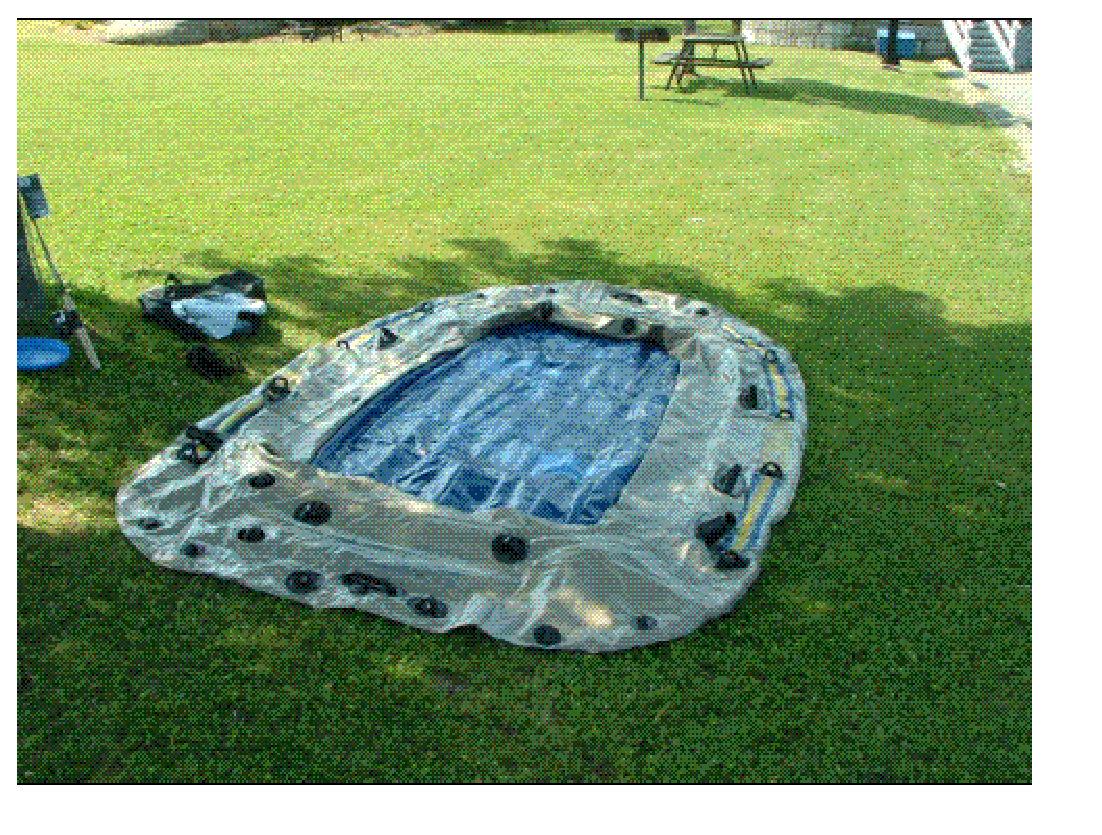
\epsfig{file=fig1.eps,width=3.5in}
Which one of the following is missing in it?
PTC-MULTICHOICE-USER( Not any of aboves. )
   PTC-CHOICE (0)An air-boat
   PTC-CHOICE (0)Lawn
   PTC-CHOICE( 0 )A frisbee
   PTC-CHOICE (1 )An airplane
   PTC-CHOICE (1 )A truck
   PTC-CHOICE( 0 )A table
PTC-MULTICHOICE-USER-END

\vspace{0.3in}
PTC-QUESTION-END




PTC-QUESTION(26;12.4;4;0)
In a hotel, the possiblity of PTC-LLL(smoking; non-smoking) customer is
$a = PTC-RRR(0.010;1.0;0.010)$, and the possiblity of PTC-LLL(equal or above 30
years old; under 30 years old) customer is $ b = PTC-RRR(0.0200;1.0;0.0200)$.
Please calculate the possiblity of PTC-PRINT-IN(1;.NOT.) and PTC-PRINT-IN(3;
.NOT.) customer.

PTC-SOLUTION
Since the possiblity of PTC-PRINT-IN(1) customer is $ a = PTC-PRINT-IN(2) $,
and the possiblity of PTC-PRINT-IN(3) customer is $ b = PTC-PRINT-IN(4) $,
the possiblity of PTC-PRINT-IN(1;.NOT.) customer is $ c = 1.0 - a = 1.0 -
PTC-PRINT-IN(2)
= PTC-PRINT-OUT(1;3) $ and the possiblity of PTC-PRINT-IN(3;.NOT.)
customer is $ d = 1.0 - b = 1.0 - PTC-PRINT-IN(4) = PTC-PRINT-OUT(2;4)  $.
So the possibility of PTC-PRINT-IN(1;.NOT.) and PTC-PRINT-IN(3;.NOT.)
customer is $ c \times d = PTC-PRINT-OUT(3;3) $.

PTC-SOLUTION-END

PTC-ANSWER
The possibility of PTC-PRINT-IN(1;.NOT.) and PTC-PRINT-IN(3;.NOT.)
customer is $ (1-a)(1-b) = PTC-PRINT-OUT(3;3) $.
PTC-ANSWER-END

\vspace{0.3in}
PTC-QUESTION-END



PTC-QUESTION(27;24.5;6;0)
In a hotel, the possiblity of PTC-LLL(smoking; non-smoking) customer is
$a = PTC-RRR(0.010;1.0;0.010)$, and the possiblity of PTC-LLL(equal-or-above 30
years old; under 30 years old) customer is $ b = PTC-RRR(0.0200;1.0;0.0200)$.
Please fill the following form.

\noindent
 \begin{tabular}{|l|l|}
 \hline
         Customer & Possibility \\
 \hline
   PTC-PRINT-IN(1;.TRUE.)  and  PTC-PRINT-IN(3;.TRUE.)  & \\
 \hline
   PTC-PRINT-IN(1;.TRUE.)  and  PTC-PRINT-IN(3;.FALSE.) & \\
 \hline
   PTC-PRINT-IN(1;.FALSE.) and  PTC-PRINT-IN(3;.TRUE.)  & \\
 \hline
   PTC-PRINT-IN(1;.FALSE.) and PTC-PRINT-IN(3;.FALSE.) & \\
 \hline
 \end{tabular}



PTC-SOLUTION
Since the possiblity of PTC-PRINT-IN(1) customer is $ a = PTC-PRINT-IN(2) $,
and the possiblity of PTC-PRINT-IN(3) customer is $ b = PTC-PRINT-IN(4) $,
the possiblity of PTC-PRINT-IN(1;.NOT.) customer is $ c = 1.0 - a = 1.0 -
PTC-PRINT-IN(2)
= PTC-PRINT-OUT(1;3) $ and the possiblity of PTC-PRINT-IN(3;.NOT.)
customer is $ d = 1.0 - b = 1.0 - PTC-PRINT-IN(4) = PTC-PRINT-OUT(2;4)  $.
Then

\noindent
 \begin{tabular}{|l|l|}
 \hline
         Customer & Possibility \\
 \hline
   PTC-PRINT-IN(1;.TRUE.)  and PTC-PRINT-IN(3;.TRUE.)  &
  $PTC-PRINT-OUT(3;3) \times PTC-PRINT-OUT(5;4) = PTC-PRINT-OUT(7; 3)$ \\
 \hline
   PTC-PRINT-IN(1;.TRUE.)  and PTC-PRINT-IN(3;.FALSE.) &
  $PTC-PRINT-OUT(3;3) \times PTC-PRINT-OUT(6;4) = PTC-PRINT-OUT(8; 3)$ \\
 \hline
   PTC-PRINT-IN(1;.FALSE.) and PTC-PRINT-IN(3;.TRUE.)  &
  $PTC-PRINT-OUT(4;3) \times PTC-PRINT-OUT(5;4) = PTC-PRINT-OUT(9; 3)$ \\
 \hline
   PTC-PRINT-IN(1;.FALSE.) and PTC-PRINT-IN(3;.FALSE.) &
  $PTC-PRINT-OUT(4;3) \times PTC-PRINT-OUT(6;4) = PTC-PRINT-OUT(10;3)$ \\
 \hline
 \end{tabular}

\noindent
And the total summation of all possibilities is $ PTC-PRINT-OUT(11;4) $.


PTC-SOLUTION-END

PTC-ANSWER

\noindent
 \begin{tabular}{|l|l|}
 \hline
         Customer & Possibility \\
 \hline
   PTC-PRINT-IN(1;.TRUE.)  and PTC-PRINT-IN(3;.TRUE.) &
  $PTC-PRINT-OUT(7; 3)$ \\
 \hline
   PTC-PRINT-IN(1;.TRUE.)  and PTC-PRINT-IN(3;.FALSE.) &
  $PTC-PRINT-OUT(8; 3)$ \\
 \hline
   PTC-PRINT-IN(1;.FALSE.) and PTC-PRINT-IN(3;.TRUE.) &
  $PTC-PRINT-OUT(9; 3)$ \\
 \hline
   PTC-PRINT-IN(1;.FALSE.) and PTC-PRINT-IN(3;.FALSE.) &
  $PTC-PRINT-OUT(10;3)$ \\
 \hline
 \end{tabular}

\noindent
 And the total summation of all possibilities is $ PTC-PRINT-OUT(11;4) $.

PTC-ANSWER-END

\vspace{0.3in}
PTC-QUESTION-END



PTC-QUESTION(28;67.2;7;0)
What is the operation between $a=PTC-III(1;10;2)$ and $b=PTC-III(2;10;2)$:
$a$ PTC-SSS($+$;$-$;$\times$;$\div$) $b=?$ Please also calculate it.
PTC-ANSWER
PTC-PRINT-IN(1);

PTC-PRINT-IN(2);

The operation is PTC-PRINT-OUT(1) and the result is
$PTC-PRINT-OUT(2;5)$.

PTC-ANSWER-END

\vspace{0.3in}
PTC-QUESTION-END



PTC-CHOOSE-END


PTC-QUESTION(50;40.0;8;1)

An object is subjected to an external net force $\mathbf{f}=
PTC-VVV (20.0; 101.0; 10.0; 2.0; 10.1; 1.0;-2000.0; -10001.0; -1000.0)N$.
Its mass is known as $m=PTC-RRR (50.0; 60.1; 2.0) kg$.
PTC-SWITCH-ON(1)
  Please choose the correct accelaration from the following choices.
  PTC-MULTICHOICE-AUTO(4;)
  The accelaration is $ PTC-CHOICES (1;
    3;0.3;-5.0; 5.0; -2.0; 2.0;
    2;0.3;-5.0; 5.0; -2.0; 2.0;
    5;0.3;-5.0; 5.0; -2.0; 2.0)ms^{-2} $.
  PTC-MULTICHOICE-AUTO-END
PTC-SWITCH-ON(2)
  Please calculate the accelaration.
  \vspace{3.0in}
  PTC-ANSWER
  The accelaration is $PTC-PRINT-OUT(1;3;2;5)ms^{-2}$.
  PTC-ANSWER-END
PTC-SWITCH-OFF

PTC-SOLUTION
We will use the Newton's Second Law:

\[
\mathbf{f}=m\mathbf{a}.
\]

Since $\mathbf{f}=PTC-PRINT-IN(1)N$
and $m=PTC-PRINT-IN(2)kg$, bring them into the above equation, then we get

\begin{eqnarray*}
\mathbf{a}&=&\frac{\mathbf{f}}m  \\
&=&\frac{PTC-PRINT-IN(1)N}{PTC-PRINT-IN(2)kg}  \\
&=&PTC-PRINT-OUT(1;3;2;5)ms^{-2}
\end{eqnarray*}

PTC-SOLUTION-END


\vspace{0.3in}
PTC-QUESTION-END




PTC-QUESTION(60;40.0;8;0)

$ \left( \begin{array}{ccccccccc}
 PTC-INTEGER-MATRIX(3;4;4;7;1)
 \end{array}\right) \times
\left( \begin{array}{c}
 PTC-INTEGER-MATRIX(4;1;2;2;1)
 \end{array}\right) $ =?


$ PTC-STRING-MATRIX(A;4;2; \alpha ; \beta ; \gamma ; \delta ; \epsilon ; \varepsilon ;
                   \zeta ; \eta ; \rho ; \sigma ; \Gamma ; \Delta ; \Theta ; \Lambda ;
                   \Xi ; \Upsilon ; \Phi ; \Psi ; \Omega )
 PTC-STRING-MATRIX(A;2;1; \beta ; \gamma ) $ =?

PTC-ANSWER

$\left( \begin{array}{ccccccccccccccc}
 PTC-PRINT-IN(1)
 \end{array}\right) \times
\left( \begin{array}{c}
 PTC-PRINT-IN(2)
 \end{array}\right)  =
 \left( \begin{array}{c}
 PTC-PRINT-OUT(1)
 \end{array}\right)  $

$ PTC-PRINT-IN(3)
 PTC-PRINT-IN(4)=
 PTC-PRINT-OUT(2)  $

PTC-ANSWER-END

PTC-SOLUTION
PTC-SOLUTION-END

\vspace{0.3in}
PTC-QUESTION-END



PTC-QUESTION(70;5.0;14;0)
PTC-ABSTRACT
  Quadratic Equation constructed from the following first two random (input) integers as roots,
  which of course should not show in the exam papers.
PTC-ABSTRACT-END

PTC-III (-11; 30; 4; PTC-HIDE   )  % First root
PTC-III (-31; 60; 3; PTC-HIDE)     % Second root
PTC-III (-15; 15; 2; PTC-HIDE)

Please solve the following equation:
\begin{eqnarray*}
PTC-PRINT-OUT(1) \times x^2 PTC-PRINT-OUT(2) PTC-PRINT-OUT(3)
                 \times x   PTC-PRINT-OUT(4) PTC-PRINT-OUT(5) =0
\end{eqnarray*}

PTC-ANSWER
PTC-PRINT-IN(1), PTC-PRINT-IN(2)

PTC-ANSWER-END

PTC-SOLUTION
Roots to the equation
\begin{eqnarray*}
PTC-PRINT-OUT(1) \times x^2 PTC-PRINT-OUT(2) PTC-PRINT-OUT(3)
                 \times x   PTC-PRINT-OUT(4) PTC-PRINT-OUT(5) =0
\end{eqnarray*}
are PTC-PRINT-IN(1) and PTC-PRINT-IN(2) .

Let us verity PTC-PRINT-IN(1) first:
$ PTC-PRINT-OUT(1) \times x^2 PTC-PRINT-OUT(2) PTC-PRINT-OUT(3)
                 \times x   PTC-PRINT-OUT(4) PTC-PRINT-OUT(5)
  =PTC-PRINT-OUT(6)+(PTC-PRINT-OUT(7))+(PTC-PRINT-OUT(5))
  =PTC-PRINT-OUT(8)+(PTC-PRINT-OUT(5))
  =PTC-PRINT-OUT(9)
$

Then verity PTC-PRINT-IN(2):
$ PTC-PRINT-OUT(1) \times x^2 PTC-PRINT-OUT(2) PTC-PRINT-OUT(3)
                 \times x   PTC-PRINT-OUT(4) PTC-PRINT-OUT(5)
  =PTC-PRINT-OUT(10)+(PTC-PRINT-OUT(11))+(PTC-PRINT-OUT(5))
  =PTC-PRINT-OUT(12)+(PTC-PRINT-OUT(5))
  =PTC-PRINT-OUT(13)
$

PTC-SOLUTION-END

\vspace{0.3in}
PTC-QUESTION-END



PTC-EXAM-TAIL
Here are still some constants for use:
PTC-CONSTANT-TABLE-HEAD
PTC-CONSTANT-TABLE-LINE (12 ;-1                   )
PTC-CONSTANT-TABLE-LINE (3 ;4               )
PTC-CONSTANT-TABLE-TAIL
Thank you very much for answering these questions!

{\textbf{\large{Please be advised}}} that in this paper there are questions from
PTC-PRINT-PARAMETER(PAPER).1 through
PTC-PRINT-PARAMETER(PAPER).PTC-PRINT-PARAMETER(TOTAL-QUESTIONS).
And any one of them may contain more than one sub-question, thus the total number
of sub-questions here is around PTC-PRINT-PARAMETER(GLOBAL-SUBQUESTIONS), of which
PTC-PRINT-PARAMETER(GLOBAL-REQUIRED-SUBQUESTIONS) should be answered.

PTC-EXAM-TAIL-END


\end{document}
